\chapter{Differential systems and Stokes filtered local systems of pure Gaussian type}

In this chapter we begin by introducing differential systems of pure Gaussian type as invented by C. Sabbah in \cite{Sabbah_2016}. 
Nevertheless our primary objective in this section is to define Stokes filtered local systems and Stokes data. Their usefulness will become apparent at the end of the chapter where we will formulate a Riemann-Hilbert correspondence that links differential systems of pure Gaussian type with Stokes filtered local systems of pure Gaussian type.

\section{Differential systems of pure Gaussian type}\label{DifferentialGauss}

The study of partial differential systems can be approached algebraically using the theory of $\Dc$-modules. This will be our method for investigating differential systems of pure Gaussian type. Therefore, we will start by considering $\Dc$-modules to define differential systems of pure Gaussian type afterwards. We follow (\cite{Sabbah_2016}, chapter 1).
\newline 


We consider the projective line $\P^1$ with an affine open covering $\P^1 = \A^1_t \cup \A^1_{t'}$ with $t = \frac{1}{t'}$ on the intersection.

\begin{lem}\label{module with connection and D module}
A left $\Dc$-module is a $\C[t]$-module with $\C$-linear connection and vice versa.
\end{lem}

\begin{proof}
Let $M$ be a $\C[t]$-module with connection $\nabla: M \to \C[t] \diff t \otimes_{\C[t]} M$ (cf.\ example (\ref{C-con})). Defining $\partial_t \cdot m \coloneqq \nabla(m)$ with $\nabla(m) \in M$ via the isomorphism \[ \begin{matrix}
    & \C[t] \diff t\otimes_{\C[t]} M & \to & M, \\ 
    &f \diff t \otimes m & \mapsto & fm
\end{matrix}\] we get a $\Dc$-module structure on $M$: For $t, \partial_t \in \Dc$ and $m \in M$ one has
\[
\partial_t \cdot (t \cdot m) = \nabla(tm) = \frac{\partial t}{\partial t}m + t \nabla(m) = m + t \nabla(m) = (1 + t \cdot \partial_t)(m) = (\partial_t \cdot t)(m)
\]
and 
\[
t \cdot (\partial_t \cdot m) = t \cdot (\nabla(m)) = t\nabla(m) = \nabla(tm) - \frac{\partial t}{\partial t} m = (\partial_t \cdot t -1) \cdot m = (t \cdot \partial_t) (m)
\]

as in $\Dc$ the relation $[\partial_t, t]=1$ holds and $\nabla$ is a $\C$-linear morphism satisfying the Leibnitz rule.

Conversely for a left $\Dc$-module $M$ we define 
\[
\begin{matrix}
\nabla: &M &\to &\C[t] \diff{t} \otimes_{\C[t]} M. \\ 
& m & \mapsto & 1 \diff{t} \otimes \partial_t \cdot m 
\end{matrix}
\]
$\nabla$ is $\C$-linear, as $\partial_t$ is $\C$-linear and $\nabla$ fulfills the Leibnitz rule since for any element $f \in \C[t]$ and any $ m \in M$ we have 
\begin{align*}
\nabla(fm)&  = 1 \diff{t} \otimes \partial_t \cdot fm = 1 \diff{t} \otimes (\partial_t \cdot f)m + f(\partial_t \cdot m) \\ & = 1 \diff{t} \otimes \frac{\partial f}{\partial t}m + 1 \diff{t} \otimes f (\partial_t\cdot m)  = \frac{\partial f}{\partial t} \diff{t} \otimes m + f \nabla(m).
\end{align*}
Thus $(M,\nabla)$ is a $\C[t]$-module with a $\C$-linear connection.
\end{proof}

\begin{rem}
The same holds for $\C[t,t^{-1}]$-modules (resp.\ $\C((t))$-modules) with $\C$-linear connections and $\C[t,t^{-1}]\langle \partial_t \rangle$-modules (resp.\ $\C((t))\langle \partial_t \rangle$-modules), as
\begin{itemize}
    \item $\Omega_{\C[t,t^{-1}]/\C} = \Omega_{\C[t]_{t}/\C} \overset{\ref{kaehlerloca}}{=} (\Omega_{\C[t]/\C})_{t} = (\C[t] \diff{t})_{t} = \C[t]_{t}\diff{t}$ and 
    \item $\Omega_{\C((t))/\C} = \Omega_{\C[[t]]_{t}/\C} \overset{\ref{kaehlerloca}}{=} (\Omega_{\C[[t]]/\C})_{t} = (\C[[t]]\diff{t})_{t} = \C((t)) \diff{t}$.
\end{itemize}
\end{rem}

\begin{rem}
    Let $(M, \nabla)$ be a free $\C[t]$-module of finite rank $r$ with two connections $\nabla_1, \nabla_2: M \to \Omega_{\C[t]/\C}^1 \otimes_{\C[t]} M$. Then $\nabla_1 - \nabla_2$ is $\C[t]$-linear as they both satisfy the Leibnitz rule. Therefore every connection is of the form $\nabla = \diff + A(t)\diff{t}$ with $A(t) \in \Mat_{r\times r}(\C[t])$ and 
    \[
    \begin{matrix}
    \diff{}: M \cong & \C[t]^r & \to & \C[t]^r &\cong \Omega_{\C[t]/\C} \otimes_{\C[t]} M \\
            & \begin{pmatrix} u_1(t) \\ \vdots \\ u_r(t) \end{pmatrix} & \mapsto  & \begin{pmatrix} \frac{\partial u_1}{\partial t}(t) \\ \vdots \\ \frac{\partial u_r}{\partial t}(t) \end{pmatrix} &
\end{matrix}
    \]
    being the canonical connection after choosing a basis of $\C[t]^r$. The analogous statement for $\C((t))$-modules with connections can be proven by using the same arguments.
\end{rem}


\begin{defi}
    Let $(\mathcal{M}, \nabla)$ be a meromorphic connection with $\dim (\mathcal{M}) = r$. We say $\mathcal{M}$ has a \emph{regular singular} connection if there exists an isomorphism $\psi: \mathcal{M} \to \C((t'))^r$, such that $\nabla = \diff + A(t')\diff t'$ and all entries of $A(t')$ have pole order at most 1 at $t'=0$. 
\end{defi}


\begin{ex}\label{kählerexample} For an arbitrary $f \in \C[t]$ consider
\[
\begin{matrix}
\diff{} + \diff(f):&  \C[t] &\to &\Omega_{\C[t]/\C} \otimes_{\C[t]} \C[t]. \\
& g & \mapsto & 1 \diff{t} \otimes \frac{\partial g}{\partial t} + \frac{\partial f}{\partial t} \cdot g
\end{matrix}
\]
Then $E^{f(t)} \coloneqq ( \C[t], \diff + \diff(f))$ is a $\Dc$-module as $\diff + \diff(f)$ is $\C$-linear and fulfills the Leibnitz rule:
\begin{align*}
(\diff{} + \diff(f))(gh) & = 1 \diff{t} \otimes \frac{\partial (gh)}{\partial_t} + \frac{\partial f}{\partial_t}(gh) = 1 \diff{t} \otimes \left( \frac{\partial g}{\partial t}h + g \frac{\partial h}{\partial t}\right) + \frac{\partial f}{\partial t}(gh) \\ 
& = 1 \diff{t} \otimes \frac{\partial g}{\partial t}h + 1 \diff{t} \otimes  g \frac{\partial h}{\partial t} + \frac{\partial f}{\partial t}(gh) \\ &  = \frac{\partial g}{\partial t} \diff{t} \otimes h + g\left(1 \diff{t} \otimes  \frac{\partial h}{\partial t} + \frac{\partial f}{\partial t}h\right)  
 = \frac{\partial g}{\partial t} \diff{t} \otimes h + g (\diff{}+\diff(f))(h).
\end{align*}
\end{ex}


Extending scalars of a $\Dc$-module $M$, viewed as a $\C[t]$-module with connection (cf.\ \ref{module with connection and D module}), to a $\C[t,t^{-1}]$-module $M'\coloneqq M \otimes_{\C[t]} \C[t,t^{-1}]$ we obtain a $\C[t',t'^{-1}]\langle \partial_{t'} \rangle$-module via 
\[
    (t',m) \mapsto t^{-1}m; ~~ 
    (t'^{-1},m) \mapsto tm ~\text{ and }~
    (\partial_{t'},m) \mapsto (-t^2\partial_t)\cdot m.
\]

\begin{ex}\label{GaussiantypeBsp}
The extension to $\C[t',t'^{-1}]$ of the $\Dc$-module we considered in example (\ref{kählerexample}) gives us the $\C[t',t'^{-1}]\langle \partial_{t'} \rangle$-module 
\[
E^{f(t'^{-1})} = (\C[t',t'^{-1}], \diff{}+\diff(f(t'^{-1}))).
\]
Further extending $\C[t',t'^{-1}]$ to $\C((t'))$ we get a $\C((t'))\langle \partial_{t'} \rangle$-module  
\[
\mathcal{E}^{f(t'^{-1})} \coloneqq E^{f(t'^{-1})} \otimes_{\C[t',t'^{-1}]} \C((t')) = (\C((t')), \diff + \diff(f(t'^{-1}))).
\]
\end{ex}

Now we can give the definition for differential systems of pure Gaussian type:

\begin{defi}\label{Gaussian type systems}
    Let $C \subseteq \C^\times$ be a non-empty, finite subset. A differential system of \emph{pure Gaussian type} $C$ is a free $\C[t]$-module $M$ of finite rank $r$ together with a connection $\nabla = \diff +A(t)\diff{t}$ with $A(t) \in \Mat_{r \times r}(\C[t])$ so that for the $\C[t,t^{-1}]$-module $M' \coloneqq M \otimes_{\C[t]} \C[t,t^{-1}]$ one has 
    \[
    (M' \otimes_{\C[t',t'^{-1}]} \C((t')), \nabla) \cong \bigoplus_{c \in C}(\mathcal{E}^{-\frac{c}{2t'^2}} \otimes_{\C((t'))} R_c) 
    \]
    with $\mathcal{E}^{-\frac{c}{2t'^2}} = (\C((t')), \diff + \frac{c}{t'^3})$ and $R_c$ is a finite dimensional $\C((t'))$-vector space with regular singular connection.
\end{defi}

\begin{rem}
    In definition (\ref{Gaussian type systems}), $\mathcal{E}^{-\frac{c}{2t'^2}}$ is given by $E^{f(t'^{-1})} \otimes_{\C[t',t'^{-1}]} \C((t'))$ for the polynomial $f(t) = -\frac{1}{2}ct^2 \in \C[t]$ as in example (\ref{GaussiantypeBsp}). Furthermore, a differential system of pure Gaussian type $C$ is by definition purely irregular at infinity of irregularity $2r$ (see \cite{Sabbah_2016}, chapter 1).
\end{rem} 

\begin{defi}
    Let $C \subseteq \C^\times$ be a non-empty, finite subset. The category $\Mod(C)$ of differential systems of pure Gaussian type $C$  is the full subcategory of $\Conn(\C[t])$ where the objects are differential systems of pure Gaussian type.
\end{defi}


\section{Stokes data of Gaussian type}
Having given a formal definition of differential systems of pure Gaussian type, we now focus on defining Stokes filtered local systems and the category of Stokes data in this section. In order to do so, we mostly follow (\cite{Sabbah_2016}, chapter 2) and (\cite{Sabbah_StokesStructures}, chapter 2). 

\subsection{Stokes directions}
To get to the definition of a Stokes filtration for a local system, we first have to establish Stokes directions.
\newline

Let $\k$ be a field and $\Lo$ be a local system of finite dimensional $\k$-vector spaces on the unit circle $S^1 \subseteq \C$ with coordinate $e^{i\theta}$. With $\theta \in S^1$ we abbreviate $e^{i\theta}\in S^1$. On $\C$ we define a partial order for each direction $\theta \in S^1$ as follows: For any $c \in \C$ we set
\[
c \leq_\theta 0 ~:\Longleftrightarrow~c = 0 ~ \text{ or }  \arg(c) - 2 \theta \in \left( \frac{\pi}{2}, \frac{3\pi}{2}\right) \mod 2 \pi.
\]
Then for $c_1, c_2 \in \C$ we set $c_1 \leq_\theta c_2$ if and only if $c_1 -c_2 \leq_\theta 0$. 

\begin{rem} For each $\theta \in S^1$, the relation $\leq_{\theta}$ is reflexive and antisymmetric by definition. To see that $\leq_{\theta}$ is also transitive, we have to check that for two complex numbers $z_1,z_2 \in \C$ with $z_1 \leq_\theta 0$ and $0 \leq_\theta z_2$, one has $z_1 \leq_\theta z_2$. In order to prove that, it is sufficient to show that for $z_1,z_2 \in \C$ with $\arg(z_1),\arg(z_2) \in (\phi, \phi+\pi)$ for some $\phi \in [0,2\pi)$, then $\arg(z_1+z_2) \mod 2\pi \in (\phi,\phi+\pi)$. One can prove this by using the rotation matrices \[R_{2\pi-\phi} = \begin{pmatrix}
    \cos(2\pi-\phi) & -\sin(2\pi-\phi) \\
    \sin(2\pi-\phi) & \cos(2\pi-\phi)
\end{pmatrix} \text{ and } R_{\phi}= \begin{pmatrix}
    \cos(\phi) & -\sin(\phi) \\
    \sin(\phi) & \cos(\phi),
\end{pmatrix}\] that rotate a complex number (considered as a vector in $\R^2$) counterclockwise by the angle $2\pi-\phi$ (resp.\ $\phi$) and the fact that if $\im(z_1) > 0$ and $\im(z_2)>0$, then $\im(z_1+z_2) >0$. Thus, $\leq_{\theta}$ is indeed a partial order.
\end{rem}

Furthermore we define a strict partial order on $\C$ for each $\theta \in S^1$ by setting $c_1 <_\theta c_2 $ if and only if $c_1 \leq_\theta c_2$ and $c_1 -c_2 \neq 0$ for two complex numbers $c_1,c_2 \in \C$.


\begin{lem}\label{relation open}
Let $\theta \in S^1$ be an arbitrary direction and $c \in \C$ be a complex number with $c \leq_{\theta} 0$. 
   Then there exists an open neighbourhood $U \subseteq S^1$ of $\theta$, so that $c \leq_{\theta'} 0$ holds for any $\theta' \in U$.
\end{lem}   
\begin{proof} For $c \in \C$ with $c \leq_{\theta} 0$, we have either $c = 0$ or $c <_{\theta}0$.
    In the case $c = 0$ we can set $U = S_1$. Thus let $c$ be a complex number with $c <_{\theta} 0$. Then by definition of $<_{\theta}$ we have 
    \begin{align*}
        \arg(c) - 2 \theta & \in \left(\frac{\pi}{2}, \frac{3\pi}{2}\right) \mod 2 \pi \\
        \Longleftrightarrow \theta &\in \left(\frac{2\arg(c)-3\pi}{4}, \frac{2\arg(c)-\pi}{4}\right) \mod 2\pi.
    \end{align*}
    Therefore there is a $k \in \Z$, so that $\theta \in \left(\frac{2\arg(c)-3\pi}{4} + k2\pi, \frac{2\arg(c)-\pi}{4}+k2\pi\right)\subseteq S^1$. Setting $U \coloneqq \left(\frac{2\arg(c)-3\pi}{4} + k2\pi, \frac{2\arg(c)-\pi}{4}+k2\pi\right)$ proves the statement, since for any $\theta' \in U$ the computation above implies that $c \leq_{\theta'} 0$.
\end{proof}
Due to lemma (\ref{relation open}), we also say that the relation $\leq_{\theta}$ is open with respect to $\theta$.
\begin{rem}
    One can check that $c\leq_{\theta} 0$ holds if and only if $\exp(\frac{c}{2t'^2})$ has moderate growth on some open neighbourhood of $t'=re^{i\theta}$ for $r \to 0$. For details see (\cite{Sabbah_StokesStructures}, example 1.4).
\end{rem}


\begin{nota}
    For $c_1, c_2 \in \C$ we define 
    \begin{align*}
    S_{c_1 \leq c_2}^1 & \coloneqq \{\theta \in S^1 \mid c_1 \leq_\theta c_2\} \subseteq S^1 \text{ and }\\ 
    S_{c_1 < c_2}^1 & \coloneqq \{ \theta \in S^1 \mid c_1 <_\theta c_2 \} \subseteq S^1.
    \end{align*}
    Lemma (\ref{relation open}) shows that $S_{c_1 \leq c_2}^1$ and $S_{c_1 < c_2}^1$ are open in $S^1$, therefore the inclusions $j_{c_1\leq c_2}: S^1_{c_1 \leq c_2} \xhookrightarrow{} S^1$ and $j_{c_1 < c_2}:S^1_{c_1 < c_2} \xhookrightarrow{} S^1$ are open. With 
    \[
        \beta_{c_1 \leq c_2}  \coloneqq (j_{c_1 \leq c_2})_!j^{-1}_{c_1 \leq c_2}: \Sh_{S^1} \to \Sh_{S^1}
    \]
    we denote the functor that restricts a sheaf on $S^1$ to the open set $S^1_{c_1 \leq c_2}$  and extends it by 0. Analogously we define $\beta_{c_1 < c_2} \coloneqq  (j_{c_1 < c_2})_!j^{-1}_{c_1 < c_2}$.
\end{nota}

Recall that for a topological space $X$ and an open inclusion $j:U \xhookrightarrow{} X$ the functor $j_!: \Sh_{U} \to \Sh_X$ maps a sheaf $\mathcal{F}$ on $U$ to the sheafification of the presheaf $\mathcal{F}'$ on $X$ that is given as follows. For an open set $V \subseteq X$ one has
\[
 \mathcal{F}': V \mapsto \mathcal{F}'(V) = \begin{cases}
    \mathcal{F}(V) & \text{ if } V \subseteq U, \\
    0 &\text{ if } V \not\subseteq U.
\end{cases}
\]

\begin{rem}
    Let $X$ be a topological space and let $j:U \xhookrightarrow{} X$ be the inclusion of an open subset. Then the functor $j_!$ is left adjoint to $j^{-1}$.
    Thus for each $\mathcal{G} \in \Sh_{S^1}$ one has a morphism of sheaves $\epsilon_{\mathcal{G}}:\beta_{c_1 \leq c_2}(\mathcal{G}) \to \mathcal{G}$ given by the counit of the adjunction. Moreover, this is a monomorphism of sheaves as for each $\theta \in S^1$ the stalk $\beta_{c_1 \leq c_2}(\mathcal{G})_\theta$ is given by
    \[
        \beta_{c_1 \leq c_2}(\mathcal{G})_\theta = \begin{cases}
            \mathcal{G}_\theta &\text{ if } \theta \in S_{c_1 \leq c_2}, \\
            0 &\text{ if } \theta \not\in S_{c_1 \leq c_2}.
        \end{cases}
    \]
    For details see (\cite{Hart}, chapter 2).
\end{rem}

We can now define Stokes directions.

\begin{defi}
   Let $c_1,c_2 \in \C$ be two complex numbers. A direction $\theta \in S^1$ with $\theta \not\in S_{c_1 \leq c_2}^1$ and $\theta \not\in S_{c_2 \leq c_1}^1$ is called a \emph{Stokes direction} of $(c_1, c_2)$. The set of Stokes directions of $(c_1,c_2)$ is denoted by $\St(c_1,c_2)$.
\end{defi}

To calculate the set of Stokes directions of a given pair of two complex numbers, we use the following lemma.

\begin{lem}\label{StokesDirections}
    Let $c_1,c_2 \in \C$ with $c_1 \neq c_2$. Then there are exactly four Stokes directions of $(c_1,c_2)$. Moreover all Stokes directions of $(c_1,c_2)$ differ by multiples of $\frac{\pi}{2}$, in particular
    \[
    \St(c_1,c_2) = \left\{\frac{\pi}{4}+ \frac{\arg(c_1-c_2)}{2} + \mathbb{Z}\cdot \frac{\pi}{2} \mod 2\pi\right\}
    \]
    holds.
\end{lem}
\begin{proof}
Let $c_1,c_2 \in \C$ with $c_1 \neq c_2$. Define $\phi \coloneqq \arg(c_1 -c_2) \in [0, 2\pi)$. Then $\arg(c_2-c_1) = \phi+\pi \mod 2\pi$ and therefore $c_1 \not\leq_{\theta} c_2$ and $c_2 \not\leq_{\theta} c_1$ only holds if
    \[
    \phi - 2 \theta \in \left[0, \frac{\pi}{2}\right] \cup \left[\frac{3\pi}{2}, 2\pi\right) \mod 2\pi ~\text{ and }~ \phi+\pi - 2 \theta \in \left[0, \frac{\pi}{2}\right] \cup \left[\frac{3\pi}{2}, 2\pi\right) \mod 2\pi.
    \] Hence, $\theta$ is a Stokes direction if $\phi -2 \theta \mod2\pi \in \{\frac{\pi}{2}, \frac{3\pi}{2}\}$, which is equivalent to $\theta \mod \pi \in \{\frac{\pi}{4}+\frac{\phi}{2}, \frac{3\pi}{4}+\frac{\phi}{2}\}$. Since there are exactly four values for $\theta \in [0,2\pi)$ that satisfy the previous, there are exactly four Stokes directions of $(c_1,c_2)$. It also shows that if $\theta_0$ is a Stokes direction of $(c_1,c_2)$, then all elements of $\St(c_1,c_2)$ are of the form $\theta_\nu \coloneqq \theta_0 + \nu\frac{\pi}{2} \mod 2\pi$ for some $\nu \in \Z/4\Z$, thus \[\St(c_1,c_2) = \left\{\frac{\pi}{4}+ \frac{\phi}{2} + \mathbb{Z}\cdot \frac{\pi}{2} \mod 2\pi\right\}.\]
\end{proof}

\begin{nota}\label{connected components}
As shown in lemma (\ref{StokesDirections}), for a pair of two different complex numbers $c_1, c_2 \in \C$ there are exactly four directions in $\St(c_1,c_2)$. Hence $S^1\smallsetminus \St(c_1,c_2)$ has four connected components. Let $T(c_1,c_2)$ be the set of these components, i.e.\ for $\theta_0 \in \St(c_1,c_2)$ and $\theta_\nu \coloneqq \theta_0 + \nu\frac{\pi}{2}$ one has \[T(c_1,c_2)\coloneqq\{(\theta_\nu, \theta_{\nu+1}) \subseteq S^1 \mid \nu \in \Z/4\Z\}.\]
Since the Stokes directions differ by a multiple of $\frac{\pi}{2}$, the elements of $T(c_1,c_2)$ are open intervals of length $\frac{\pi}{2}$. Besides, using lemma (\ref{relation open}) we can observe that for every element $I \in T(c_1,c_2)$, either $c_1 \leq_{\theta} c_2$ for all $\theta \in I$ or $c_2 \leq_{\theta} c_1$ for all $\theta \in I$.
\end{nota}

\begin{ex}
Let $C =\{0, 1, c\}\subseteq \C$ with $\arg(c) = \phi$. Then 
\begin{itemize}
     \item $\St(0,1) = \left\{\frac{\pi}{4} + \nu \frac{\pi}{2} \mid \nu \in \Z/4\Z \right\},$
     \item $\St(0,c) = \left\{\frac{\pi}{4} + \frac{\phi}{2}+ \nu\frac{\pi}{2} \mid \nu \in \Z/4\Z\right\}$,
     \item $T(0,1) = \left\{\left(-\frac{\pi}{4}, \frac{\pi}{4}\right), \left(\frac{\pi}{4}, \frac{3\pi}{4}\right), \left(\frac{3\pi}{4}, \frac{5\pi}{4}\right), \left(\frac{5\pi}{4},\frac{7\pi}{4}\right)\right\}$ and
     \item $T(0,c) = \left\{\left(\frac{-\pi+2\phi}{4}, \frac{\pi+2\phi}{4} \right), \left(\frac{\pi+2\phi}{4}, \frac{3\pi+2\phi}{4}\right), \left(\frac{3\pi+2\phi}{4},\frac{5\pi+2\phi}{4}\right), \left(\frac{5\pi+2\phi}{4}, \frac{8\pi+2\phi}{4}\right)\right\}$.
 \end{itemize}
 
\begin{figure}[h!]
\centering
\begin{minipage}{0.48\textwidth}
\centering
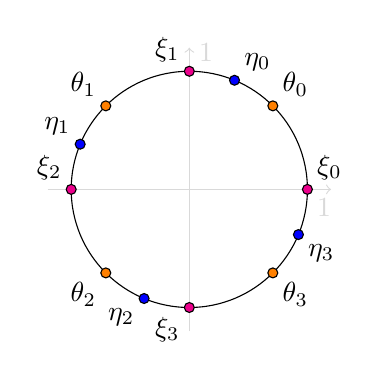
\begin{tikzpicture}[scale=0.6]
  % Gray coordinate system
  \draw[gray!30,->] (-3,0) -- (3,0) node[right] {$\re$};
  \draw[gray!30,->] (0,-3) -- (0,3) node[above] {$\im$};
  \draw[gray!30,fill=gray] (2.5,0) circle (1pt) node[below right] {1};
  \draw[gray!30,fill=gray] (0,2.5) circle (1pt) node[above right] {1};
  
  % Circle with radius 3cm
  \draw (0,0) circle (2.5cm);
  
  % First dot at angle pi/4
  \draw[fill=orange] (45:2.5cm) circle (3pt) node[above right] {$\theta_0$};
  \draw[fill=orange] (135:2.5cm) circle (3pt) node[above left] {$\theta_1$};
  \draw[fill=orange] (225:2.5cm) circle (3pt) node[below left] {$\theta_2$};
  \draw[fill=orange] (315:2.5cm) circle (3pt) node[below right] {$\theta_3$};
  \draw[fill=magenta] (90:2.5cm) circle (3pt) node[above left] {$\xi_1$};
  \draw[fill=magenta] (180:2.5cm) circle (3pt) node[above left] {$\xi_2$};
  \draw[fill=magenta] (270:2.5cm) circle (3pt) node[below left] {$\xi_3$};
  \draw[fill=magenta] (0:2.5cm) circle (3pt) node[above right] {$\xi_0$};
  \draw[fill=blue] (67.5:2.5cm) circle (3pt) node[above right] {$\eta_0$};
  \draw[fill=blue] (157.5:2.5cm) circle (3pt) node[above left] {$\eta_1$};
  \draw[fill=blue] (247.5:2.5cm) circle (3pt) node[below left] {$\eta_2$};
  \draw[fill=blue] (337.5:2.5cm) circle (3pt) node[below right] {$\eta_3$};

\end{tikzpicture}
    \captionsetup{font=small}
    \caption{$\St(0,1)$ in orange, $\St(0,c)$ in blue and $\St(1,c)$ in pink for $c = 1+i$.}
\end{minipage}
\hfill
\begin{minipage}{0.48\textwidth}
\centering
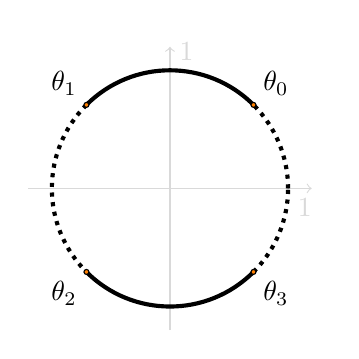
\begin{tikzpicture}[scale=0.6]
    \draw[gray!30,->] (-3,0) -- (3,0) node[right] {$\re$};
    \draw[gray!30,->] (0,-3) -- (0,3) node[above] {$\im$};
    \draw[gray!30,fill=gray] (2.5,0) circle (1pt) node[below right] {1};
    \draw[gray!30,fill=gray] (0,2.5) circle (1pt) node[above right] {1};

     % Intervalle:
   \draw[line width=1.5pt]  (45:2.5cm) arc (45:135:2.5cm);
   \draw[dotted, line width=1.5pt] (135:2.5cm) arc (135:225:2.5cm);
   \draw[line width=1.5pt] (225:2.5cm) arc (225:315:2.5cm);
   \draw[dotted, line width=1.5pt] (315:2.5cm) arc (315:360:2.5cm);
   \draw[dotted, line width=1.5pt] (0:2.5cm) arc (0:45:2.5cm);

   \draw[fill=orange]  (45:2.5cm) circle (1.5pt) node[above right] {$\theta_0$};
  \draw[fill=orange] (135:2.5cm) circle (1.5pt) node[above left] {$\theta_1$};
  \draw[fill=orange] (225:2.5cm) circle (1.5pt) node[below left] {$\theta_2$};
  \draw[fill=orange] (315:2.5cm) circle (1.5pt) node[below right] {$\theta_3$};
\end{tikzpicture}
    \captionsetup{font=small}
    \caption{The sets $S^1_{0 \leq 1}$, outlined by the dotted line and $S^1_{1 \leq 0}$ outlined by the full line.}
\end{minipage}


\end{figure}
\end{ex}

\subsection{Stokes filtered local systems}

Now, having seen Stokes directions, we can give the definitions for (pre-)Stokes filtered local systems. To do this, we specify the contents of chapter 2 of \cite{Sabbah_StokesStructures} to fit our framework, namely we define Stokes filtrations of local systems that are of Gaussian type.

\begin{defi}
A \emph{pre-Stokes filtered local system of Gaussian type} is a pair $(\Lo, (\Lo_{\leq c})_{c\in\C})$, where 
\begin{enumerate}
    \item $\Lo$ is a local system of finite dimensional $\k$-vector spaces on $S^1$ and
    \item $(\Lo_{\leq c})_{c \in \C}$ is a family of subsheaves of $\Lo$ in such way that for any $c_1, c_2 \in \C$ and $\theta \in S^1$ the implication 
    \[
    c_1 \leq_\theta c_2 \Longrightarrow \Lo_{\leq c_1, \theta} \subseteq \Lo_{\leq c_2, \theta}
    \]
    holds and forms an exhaustive increasing filtration of $\Lo_\theta$. 
\end{enumerate}
We say that $(\Lo_{\leq c})_{c \in \C}$ is a \emph{pre-Stokes filtration of Gaussian type} of $\Lo$.
\end{defi} 

\begin{ex}
    Consider the constant sheaf $\Lo \coloneqq \underline{\k}_{S^1}$ and for each $c \in \C$ the subsheaf $\Lo_{\leq c} \coloneqq \beta_{0 \leq c}(\underline{\k}_{S^1})$. Then $(\Lo,(\Lo_{\leq c})_{c \in \C})$ is a pre-Stokes filtered local system of Gaussian type since $\Lo$ is a local system and for any $\theta \in S^1, c \in \C$ we have
    \[
    \Lo_{\leq c, \theta} = \beta_{0 \leq c}(\underline{\k}_{S^1})_\theta = \begin{cases} \k & \text{ if } 0 \leq_{\theta} c, \\ 0 & \text{ if } 0 \not\leq_{\theta} c.\end{cases}
    \]
    Transitivity of $\leq_{\theta}$ implies the property $c_1 \leq_{\theta} c_2 \Longrightarrow \Lo_{\leq c_1,\theta} \subseteq \Lo_{\leq_{c_2},\theta}$. Since $\Lo_{\leq 0} = \Lo$ the filtration of $\Lo_\theta$ is exhaustive.
\end{ex}

Let $(\Lo,(\Lo_{\leq c})_{c\in\C})$ be a pre-Stokes filtered local system of Gaussian type.
For any $\theta \in S^1$ and $c \in \C$ the $\k$-vector spaces \[\Lo_{< c, \theta} \coloneqq \sum_{c' <_\theta c} \Lo_{\leq c', \theta}\] glue together to a subsheaf $\Lo_{< c}$ of $\Lo_{\leq c}$, given by 
\[\Lo_{< c}(U) \coloneqq \left\{ \sigma \in \Lo(U) ~ \Big\vert ~ [\sigma]_{\theta} \in \sum_{c' <_\theta c} \Lo_{\leq c', \theta} \text{ for all } \theta \in U\right\}\] for an open subset $U \subseteq S^1$, because $\leq_{\theta}$ is open with respect to $\theta$. By  $\gr_c \Lo$ we denote the quotient sheaf $\Lo_{\leq c}/\Lo_{< c}$. Then by
\[
\gr \Lo \coloneqq \bigoplus_{c \in \C}\gr_c\Lo=\bigoplus_{c\in \C} \Lo_{\leq c}/\Lo_{< c}
\] we get a graded sheaf. Furthermore for any $c \in \C$ and $\theta \in S^1$ the $\k$-vector spaces
\[\gr \Lo_{\leq c, \theta} \coloneqq \bigoplus_{c' \leq_\theta c} \gr_{c'}\Lo_\theta\] glue together to a subsheaf $\gr\Lo_{\leq c}$ of $\gr\Lo$ that is given by 
\[
\gr\Lo_{\leq c} = \bigoplus_{c' \in \C}\beta_{c' \leq c} (\gr_{c'}\Lo).
\]

Now we can give the definition of a Stokes filtration of Gaussian type.

\begin{defi}\label{Stokesfiltration} Let $\Lo$ be a local system of finite dimensional $\k$-vector spaces on $S^1$.
    A pre-Stokes filtration of Gaussian type $(\Lo_{\leq c})_{c\in\C}$ of $\Lo$ is a \emph{Stokes filtration of Gaussian type} if it satisfies the following properties:
    \begin{enumerate}
        \item $\gr_c \Lo$ is an object in $\Loc_{S^1}$ for any $c \in \C$.
        \item $(\Lo, (\Lo_{\leq c})_{c \in \C})$ is locally isomorphic to $(\gr\Lo, (\gr\Lo_{\leq c})_{c \in \C})$, i.e.\ for any direction $\theta \in S^1$ there is a neighbourhood $U \subseteq S^1$ of $\theta$ and an isomorphism of local systems $\Lo_{\vert U} \to \gr\Lo_{\vert U}$. Moreover for any $\theta \in S^1$ and $c \in \C$ there is an open neighbourhood $U_c \subseteq S^1$ of $\theta$ and an isomorphism $\Lo_{\leq c \vert_{U_c}} \to \gr\Lo_{\leq c\vert_{U_c}}$.
    \end{enumerate}
    We also say that $(\Lo, (\Lo_{\leq c})_{c \in \C})$ is a Stokes filtered local system of Gaussian type.
\end{defi}

We can classify Stokes filtered local systems using the following insight:

\begin{lem}
    Let $(\Lo, (\Lo_{\leq c})_{c \in \C})$ be a Stokes filtered local system of Gaussian type. Then the set $\left\{c \in \C \mid \gr_c\Lo \neq 0\right\}$, called \emph{the set of exponential factors} of the Stokes filtration, is finite.
\end{lem}
\begin{proof}
    Since $(\Lo, (\Lo_{\leq c})_{c \in \C})$ is a Stokes filtered local system of Gaussian type,  $\Lo_\theta$ has finite dimension for every $\theta \in S^1$. Therefore there are only finitely many $c \in \C$ with $\Lo_{\leq \tilde{c}, \theta} \subsetneq \Lo_{\leq c, \theta}$ for all $\tilde{c} \in \C$ with $\tilde{c} <_{\theta} c$, as this forms a filtration of $\Lo_\theta$. Hence for all except a finite number of $c \in \C$, there is a $\tilde{c} \in \C$ with $\tilde{c}<_{\theta} c$ and $\Lo_{\leq \tilde{c}, \theta} = \Lo_{\leq c, \theta}$. For these we have
\[
\Lo_{<c, \theta} = \sum_{\tilde{c} <_{\theta} c}\Lo_{\leq \tilde{c}, \theta} = \Lo_{\leq c, \theta},
\] and consequently $\gr_c\Lo_\theta = \Lo_{\leq c,\theta}/\Lo_{<c,\theta}$ = 0. As $\gr_c\Lo$ is a local system on $S^1$ and $S^1$ is connected we can conclude that $\gr_c\Lo = 0$ using lemma (\ref{same dimension}). Thus the set of exponential factors $\{c \in \C \mid \gr_c\Lo\neq 0\}$ is finite.  
\end{proof}
 

\begin{nota}
    Let $(\Lo, (\Lo_{\leq c})_{c \in \C})$ be a Stokes filtered local system of Gaussian type and $C \subseteq \C$ be a finite subset. We say $(\Lo, (\Lo_{\leq c})_{c \in \C})$ is \emph{of type $C$} if its set of exponential factors is a subset of $C$. In the following we abbreviate the notation $(\Lo, (\Lo_{\leq c})_{c \in \C})$ to $(\Lo, \Lo_{\leq \bullet})$.
\end{nota}

\begin{ex}\label{gradedLoSys}
    Let $(\Lo, \Lo_{\leq \bullet})$ be a Stokes filtered local system of Gaussian type. Given that its set of exponential factors is finite, $\gr \Lo$ is a local system. The implication 
    \[
    c_1 \leq_{\theta} c_2 \Longrightarrow \gr\Lo_{\leq c_1,\theta} \subseteq \gr\Lo_{\leq c_2, \theta} 
    \]
    follows directly form the definition of $\gr\Lo_{\leq \bullet}$.  Furthermore for an arbitrary direction $\theta \in S^1$, property 2.\ of (\ref{Stokesfiltration}) implies $\Lo_\theta \cong \gr\Lo_\theta$ and $\Lo_{\leq c, \theta} \cong \gr\Lo_{\leq c, \theta}$. As the implication $c_1 \leq_\theta c_2 \Longrightarrow \Lo_{\leq c_1,\theta} \subseteq \Lo_{\leq c_2, \theta}$
    forms an exhaustive filtration of $\Lo_{\theta}$, the same holds for $\gr\Lo_{\theta}$, so $(\gr \Lo, \gr \Lo_{\leq \bullet})$ is a pre-Stokes filtered local system of Gaussian type. Since $\gr_c(\gr \Lo) \cong \gr_c\Lo$ it follows that $(\gr\Lo_{\leq \bullet})$ fulfills the two properties of definition (\ref{Stokesfiltration}), hence $(\gr\Lo_{\leq \bullet})$ is a Stokes filtration. We also say that $(\gr\Lo, \gr\Lo_{\leq \bullet})$ is a \emph{graded Stokes filtered local system of Gaussian type}.
\end{ex}
More general we have the following: 
\begin{defi}\label{gradedLoSysDef}
    For a finite set $C \subseteq \C$ a \emph{graded Stokes filtered local system of Gaussian type $C$} is a pair $(\gr\Lo, (\gr\Lo_{\leq c})_{c \in \C})$ where for each $c \in C$ there is a local system $\gr_c\Lo$ on $S^1$ such that 
    \[\gr\Lo = \bigoplus_{c \in C} \gr_c\Lo \] and for each $c' \in \C$ 
    \[\gr\Lo_{\leq c'} = \bigoplus_{c \in C} \beta_{c \leq c'}(\gr_c\Lo).\]
\end{defi}

In chapter (\ref{DifferentialGauss}) we gave the definition of differential systems that are of \emph{pure} Gaussian type. Thus, the question arises which property Stokes filtered local systems need to fulfill to be of pure Gaussian type as well, so we can formulate the Riemann-Hilbert correspondence 
for differential systems that are of pure Gaussian type later on.

\begin{defi}
    Let $C \subseteq \C$ be a non-empty, finite subset and $(\Lo,\Lo_{\leq \bullet})$ be a Stokes filtered local system of Gaussian type $C$. We say that $(\Lo,\Lo_{\leq \bullet})$ is \emph{of pure Gaussian type} $C$ if $\Lo$ is a constant sheaf and $0 \not\in C$.
\end{defi}

To finally define the category of Stokes filtered local systems that are of Gaussian type, we have to determine morphisms within this category.

\begin{defi}
Let $(\Lo, \Lo_{\leq \bullet}), (\Lo', \Lo'_{\leq \bullet})$ be two Stokes filtered local systems of Gaussian type $C$. A \emph{morphism $\lambda: (\Lo, \Lo_{\leq \bullet}) \to (\Lo', \Lo'_{\leq \bullet})$ of (pre-)Stokes filtered local systems of Gaussian type $C$} is a morphism $\lambda\in \Hom_{\Loc_{S^1}}(\Lo, \Lo')$ satisfying $\lambda(\Lo_{\leq c})\subseteq \Lo'_{\leq c}$ for each $c \in \C$. We denote the category of Stokes filtered local systems of Gaussian type $C$ by $\LocSt(C).$

Furthermore the category of Stokes filtered local systems of pure Gaussian type $C$, indicated by $\Locpure(C)$, is the full subcategory of $\LocSt(C)$ where the objects are of pure Gaussian type $C$.
\end{defi}

\begin{rem}
    If $C'$ is a non-empty subset of the finite set $C \subseteq \C$, then $\LocSt(C')$ forms a full subcategory of $\LocSt(C)$. Furthermore if $0 \not\in C$, then $\Locpure(C')$ is a full subcategory of $\Locpure(C)$.
\end{rem}

As we will also consider the category of graded Stokes filtered local systems later on, we need to define morphisms for this category as well.

\begin{defi}\label{gradedmorphism}
    Let $(\gr\Lo, \gr\Lo_{\leq \bullet}), (\gr\Lo', \gr\Lo_{\leq \bullet}')$ be two graded Stokes filtered local systems of Gaussian type $C$. A \emph{morphism $\lambda: (\gr\Lo, \gr\Lo_{\leq \bullet}) \to (\gr\Lo', \gr\Lo_{\leq \bullet}')$ of graded Stokes filtered local systems of Gaussian type $C$} is a graded morphism of sheaves \[\lambda: \gr\Lo=\bigoplus_{c\in C}\gr_c\Lo \to \bigoplus_{c \in C}\gr_c\Lo' = \gr\Lo',\] satisfying  $\lambda(\gr\Lo_{\leq c}) \subseteq \gr\Lo_{\leq c}'$. We denote the category of graded Stokes filtered local systems by $\LocStgr(C)$.
\end{defi}

\begin{rem}
    More precisely, after decomposing $\lambda:\bigoplus_{c\in C}\gr_c\Lo \to \bigoplus_{c \in C}\gr_c\Lo'$ into blocks of morphisms of local systems \[\lambda = (\lambda_{ji}: \gr_{c_i}\Lo \to \gr_{c_j}\Lo')_{c_i,c_j \in C},\] we say $\lambda$ is graded if $\lambda_{ji} = 0$ for $c_i \neq c_j$.
\end{rem}



By definition (\ref{Stokesfiltration}) each Stokes filtered local system $(\Lo, \Lo_{\leq \bullet})$ of type $C$ is locally isomorphic to the graded Stokes filtered local system $(\gr\Lo, \gr\Lo_{\leq \bullet})$. In fact for an interval $I$ of ``correct length'', there is a unique splitting $\Lo_{\vert I} \cong \bigoplus_{c \in C}\gr_c\Lo_{\vert_I}$, that is compatible with the Stokes filtration $(\Lo_{\leq \bullet})$. In order to give the precise statement, we first need to establish what ``correct length'' means.

\begin{defi}\label{genericdirection}
Let $C \subseteq \C$ be a non-empty, finite subset. 
A direction $\theta_0 \in S^1$ is said to be \emph{generic} with respect to $C$ if $\theta_0$ is not a Stokes direction for any pair $(c,c')$ with $c\neq c'$ in $C$.
Besides, a \emph{$C$-good closed interval} $I \subseteq \R/2\pi\Z$ is a closed interval such that its interior contains exactly one Stokes direction for each pair of distinct elements $(c,c')$ in $C$.
\end{defi}

\begin{rem}
    Given that we exclusively deal with finite sets $C \subseteq \C$, and every pair of two different complex numbers offers precisely four Stokes directions, there always exists a generic direction for $C$. Moreover if $\theta_0 \in S^1$ is generic with respect to $C$, then $\theta_\nu \coloneqq \theta_0 + \nu\frac{\pi}{2}$ is generic and $[\theta_\nu, \theta_\nu + \frac{\pi}{2}]$ is a $C$-good closed interval for all $\nu\in \Z/4\Z$. Therefore we can always consider $C$-good closed intervals of the form $I = [\theta_\nu, \theta_\nu + \frac{\pi}{2}]$.
\end{rem}

\begin{ex} Let $C\coloneqq\{0,1,1+i\} \subseteq \C$. Then $\theta_0 = \frac{\pi}{16}\in S^1$ is generic with respect to $C$ and the closed interval $[\theta_0,\theta_0+\frac{\pi}{2}]$ is $C$-good.
\begin{figure}[h!]
\centering
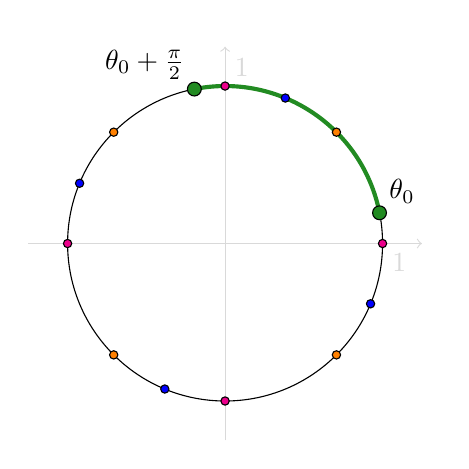
\begin{tikzpicture}
  % Gray coordinate system
  \draw[gray!30,->] (-2.5,0) -- (2.5,0) node[right] {$\re$};
  \draw[gray!30,->] (0,-2.5) -- (0,2.5) node[above] {$\im$};

  \draw[gray!30,fill=gray] (2,0) circle (1pt) node[below right] {1};
  \draw[gray!30,fill=gray] (0,2) circle (1pt) node[above right] {1};
  % Circle with radius 2.5cm
  \draw (0,0) circle (2cm);
  % First dot at angle pi/4
  \draw[ForestGreen, line width=1.5pt] (11.25:2cm) arc (11.25:101.25:2cm);
  \draw[fill=orange] (45:2cm) circle (1.5pt) node[above right] {};
  \draw[fill=orange] (135:2cm) circle (1.5pt) node[above left]{};
  \draw[fill=orange] (225:2cm) circle (1.5pt) node[below left]{};
  \draw[fill=orange] (315:2cm) circle (1.5pt) node[below right]{};
  \draw[fill=magenta] (90:2cm) circle (1.5pt) node[above left]{};
  \draw[fill=magenta] (180:2cm) circle (1.5pt) node[above left]{};
  \draw[fill=magenta] (270:2cm) circle (1.5pt) node[below left]{};
  \draw[fill=magenta] (0:2cm) circle (1.5pt) node[above right]{};
  \draw[fill=blue] (67.5:2cm) circle (1.5pt) node[above right]{};
  \draw[fill=blue] (157.5:2cm) circle (1.5pt) node[above left]{};
  \draw[fill=blue] (247.5:2cm) circle (1.5pt) node[below left]{};
  \draw[fill=blue] (337.5:2cm) circle (1.5pt) node[below right]{};
  \draw[fill=ForestGreen] (101.25:2cm) circle (2.5pt) node[above left]{$\theta_0+\frac{\pi}{2}$};
  \draw[fill=ForestGreen] (11.25:2cm) circle (2.5pt) node[above right]{$\theta_0$};
\end{tikzpicture}
    \captionsetup{font=small}
    \caption{A generic direction $\theta_0= \frac{\pi}{16}$ with respect to $C= \{0,1,1+i\}$ in green, together with the $C$-good closed interval $I = [\theta_0, \theta_0+ \frac{\pi}{2}]$. The other dots are Stokes directions of $C$ (compare to figure 3.1).}
    \label{fig C-good}
\end{figure}
\end{ex}

Using $C$-good intervals we obtain a unique splitting $\Lo_{\vert_I}\cong \bigoplus_{c \in C} \gr_c\Lo_{\vert I}$. More precisely, we get the splitting lemma:

\begin{prop}\label{splitting} Let $(\Lo, \Lo_{\leq \bullet})$ be a Stokes filtered local system of Gaussian type $C, \theta_0\in S^1$ be a generic direction with respect to $C$ and consider the $C$-good closed interval $I \coloneqq [\theta_0, \theta_0+\frac{\pi}{2}]\subseteq\R/2\pi \Z.$ Then the following properties hold:
\begin{enumerate} 
    \item There exists a unique splitting $\Lo_{\vert_I} \cong \bigoplus_{c \in C}\gr_c\Lo_{\vert_I}$ that is compatible with the Stokes filtration. With respect to this splitting, we have
    \[\Lo_{\leq c\vert_I} = \bigoplus_{c' \in C} \beta_{c' \leq c} (\gr_{c'} \Lo)_{\vert_I}.\]
    \item Let $\lambda: (\Lo, \Lo_{\leq \bullet}) \to (\Lo', \Lo'_{\leq \bullet})$ be a morphism of Stokes filtered local systems of Gaussian Type $C$. Then the morphism $\lambda_{\vert_I}$ is graded with respect to the splittings in 1.
\end{enumerate}
\end{prop}

\begin{proof}
See \cite{Hertling-Sabbah_2011}, proposition 2.2.
\end{proof}

\begin{rem}
    We want to make 2.\ of proposition (\ref{splitting}) precise. 
    
    Let $\lambda:(\Lo, \Lo_{\leq \bullet}) \to (\Lo', \Lo'_{\leq \bullet})$ be a morphism of Stokes filtered local systems. Using the unique splitting for a $C$-good closed interval $I$ we get in 1.\ of proposition (\ref{splitting}), we can decompose
    \[ \lambda_{\vert_I}: \Lo_{\vert_I} \cong \bigoplus_{c \in C}\gr_c\Lo_{\vert_I} \to \bigoplus_{c \in C}\gr_c\Lo'_{\vert_I} \cong \Lo'_{\vert_I}\]
    into blocks of morphisms of local systems
    \[
    ((\lambda_{\vert_I})_{ji}: \gr_{c_i}\Lo \to \gr_{c_j}\Lo')_{c_i,c_j \in C}.
    \]
    Then, similar to definition (\ref{gradedmorphism}), $\lambda_{\vert_I}$ is graded with respect to the splittings in 1. if  $(\lambda_{\vert_I})_{ji} =0$ for $i \neq j$.
\end{rem}

Stokes filtrations can be used to encode the Stokes structure near an irregular singular point of a differential equation in the local system (details can be found in \cite{Sabbah_StokesStructures}). In the following, we will get to know another approach to understand the Stokes structure. 

%%%%%%%%%%%%%%%%%%%%%%%%%%%%%% VIELLEICHT MIT REIN NEHMEN %%%%%%%%%%%%%%%%%%%%%%%%%%

\begin{comment}
\begin{prop} For any non-empty, finite set $C \subseteq \C$, the category $\LocSt(C)$ is abelian.
\end{prop}

\begin{proof} As a morphism $\lambda$ in $\LocSt(C)$ is a morphism in $\Loc_{S^1}$ and this category is abelian, $\ker(\lambda)$ and $\coker(\lambda)$ are local systems on $S^1$. Thus we need to find matching filtrations. Let $\lambda: (\Lo,(\Lo_{\leq \bullet})) \to (\Lo',(\Lo'_{\leq \bullet}))$ be a morphism of Stokes filtered local systems. Then for any $C$-good interval $I$, $\lambda_{\vert_I}$ is graded with respect to the unique splittings in (\ref{splitting}). This implies that on any $C$-good interval $\ker(\lambda_{\vert_I})_{\leq \bullet} = \ker(\lambda_{\vert_I}: (\Lo_{\vert_I})_{\leq \bullet} \to (\Lo_{\vert_I}')_{\leq \bullet})$
\textcolor{red}{Bisschen unklar; Denke das lasse ich raus.}
\end{proof}
\end{comment}

%%%%%%%%%%%%%%%%%%%%%%%%%%%%%%%%%%%%%%%%%%%%%%%%%%%%%%%%%%%%%%%%%%%%%%%%%%%%%%%%%%%%
\subsection{Stokes data}

In this section, our main objective is to define the category of Stokes data. This category describes Stokes structures using linear data, specifically vector spaces and linear morphisms. Moreover, Stokes filtered local systems of pure Gaussian type can be understood using the category of Stokes data. We follow the approach outlined in (\cite{Sabbah_2016}, chapter 2b) and (\cite{Hohl_Diss}, chapter 2.5).
\newline

 Let $C \subseteq \C$ be a non-empty, finite subset and $\theta_0 \in S^1$ a generic direction with respect to $C$. Then for any pair of two different elements $c,c' \in C$ we can compare $c, c'$ using $<_{\theta_0}$. In this way we get a unique numbering of $C$, satisfying $c_1 <_{\theta_0} c_2 <_{\theta_0} \dots <_{\theta_0} c_r$ with $r \in \mathbb{N}$ being the cardinality of $C$. 


 \begin{defi}\label{StokesDataDefi}
     Let $C$ be a non-empty finite subset of $\C$, $\theta_0$ a generic direction with respect to $C$ and let $\{c_1, \dots, c_r\}$ be the unique numbering of $C$ given by $\theta_0$. The \emph{category $\SD(C, \theta_0)$ of Stokes data of Gaussian type $(C,\theta_0)$} is defined by the following:
    \begin{itemize}
        \item An object $\sigma =((G_c^{(\nu)})_{c \in C}, S^{(\nu+1, \nu)})_{\nu \in \Z/4\Z}$ consists of four families of finite-dimensional $\k$-vector spaces $(G_c^{(\nu)})_{c \in C}$, together with four linear morphisms $S^{(\nu+1,\nu)}$, shown in the following diagram
        \[
         \begin{tikzcd}[row sep=1cm, column sep=0cm]
         & \bigoplus_{c \in C} G_c^{(0)} \arrow[dl, "S^{(1,0)}"'] & \\
        \bigoplus_{c \in C} G_c^{(1)} \arrow[dr, "S^{(2,1)}"'] & & \bigoplus_{c \in C} G_c^{(3)} \arrow[ul, "S^{(0,3)}" above right] \\
        & \bigoplus_{c \in C} G_c^{(2)}\arrow[ur, "S^{(3,2)}" below right] &
        \end{tikzcd}
        \]
        
        such that writing $S^{(\nu+1,\nu)}=(S^{(\nu+1,\nu)}_{ij}:G_{c_j}^{(\nu)} \to G_{c_i}^{(\nu+1)})_{i,j \in \{0,\dots,r\}}$ the following properties hold:
        \begin{itemize}
            \item $S^{(0,3)}$ and $S^{(2,1)}$ are block-upper triangular, i.e.\ $S^{(\nu+1,\nu)}_{ij}$ is zero if $i > j$ for $\nu \in \{1,3\}$.
            \item $S^{(1,0)}$ and $S^{(3,2)}$ are block-lower triangular, i.e.\ $S^{(\nu+1,\nu)}_{ij}$ is zero if $i < j$ for $\nu \in \{0,2\}$.
            \item $S_{ii}^{(\nu+1,\nu)}$ is invertible for all $i \in \{1, \dots, r\}$ and $\nu \in \Z/4\Z$.
        \end{itemize}
        \item A morphism $\lambda \in \Hom_{\SD}(\sigma, \tilde{\sigma})$ between $\sigma = ((G_c^{(\nu)})_{c \in C}, S^{(\nu+1, \nu)})_{\nu \in \Z/4\Z}$ and $\tilde{\sigma}=((\tilde{G}_c^{(\nu)})_{c \in C}, \tilde{S}^{(\nu+1, \nu)})_{\nu \in \Z/4\Z}$ is a family of four linear morphisms \[\left(\lambda^{(\nu)}:\bigoplus_{c \in C}G_c^{(\nu)}\to\bigoplus_{c \in C}\tilde{G}_c^{(\nu)} \right)_{\nu \in \Z/4\Z},\] such that writing $\lambda^{(\nu)} =(\lambda^{(\nu)}_{ij}:G_{c_j}^{(\nu)} \to \tilde{G}_{c_i}^{(\nu)})_{i,j \in \{0, \dots, r\}}$ the following properties hold:
        \begin{itemize}
            \item $\lambda^{(\nu)}_{ij}$ is zero if $i \neq j$, i.e.\ $\lambda^{(\nu)}$ is block-diagonal for every $\nu \in \Z/4\Z$.
            \item For any $\nu \in \Z/4\Z$, one has $\tilde{S}^{(\nu+1,\nu)}\lambda^{(\nu)} = \lambda^{(\nu+1)}S^{(\nu+1, \nu)}$.
        \end{itemize}
        The composition of two morphisms of Stokes data $\lambda \in \Hom_{\SD(C,\theta_0)}(\sigma_1, \sigma_2)$ and $\mu \in \Hom_{\SD(C, \theta_0)}(\sigma_2, \sigma_3)$ is given by $\mu\circ\lambda = (\mu^{(\nu)}\circ\lambda^{(\nu)})_{\nu \in \Z/4\Z}$ where $\mu^{(\nu)}\circ \lambda^{(\nu)}$ is the composition in $\Vect_\k$. 
    \end{itemize}
 \end{defi}

 \begin{rem}
    As $S_{ii}^{(\nu+1,\nu)}$ is invertible for every $c_i \in C$ and $\nu \in \Z/4\Z$, we get $\dim G_{c_i}^{(\nu)} = \dim G_{c_i}^{(\nu+1)}$. Furthermore, by definition (\ref{StokesDataDefi}), $S^{(\nu+1,\nu)}$ is a block-upper (resp.\ block-lower) matrix with invertible matrices on its diagonal. Therefore $S^{(\nu+1,\nu)}$ is invertible.
\end{rem}

Again, we also want the notion of Stokes data that are of \emph{pure} Gaussian type.

 \begin{defi} Let $C \subseteq \C^\times$ be a non-empty, finite subset and let $\theta_0$ be a generic direction with respect to $C$. Then the \emph{category $\SDpure(C,\theta_0)$ of Stokes data of pure Gaussian type $(C,\theta_0)$} is the full subcategory of $\SD(C,\theta_0)$ where the objects $\sigma = ((G_c^{(\nu)})_{c \in C}, S^{(\nu+1, \nu)})_{\nu \in \Z/4\Z}$ satisfy 
 \[
S^{(0,3)}S^{(3,2)}S^{(2,1)}S^{(1,0)} = \id_{\bigoplus_{c\in C}G_c^{(0)}} \in \Hom_{\Vect_\k}\left(\bigoplus_{c\in C}G_c^{(0)},\bigoplus_{c\in C}G_c^{(0)}\right).
 \]
 \end{defi}


\begin{prop}\label{SDabelsch} Let $C \subseteq \C$ be a non-empty finite subset and $\theta_0 \in S^1$ a generic direction with respect to $C$. The category $\SD(C,\theta_0)$ of Stokes data of Gaussian type $(C, \theta_0)$ is abelian.
\end{prop}

\begin{proof} Since $\Vect_\k$ is an additive category, $\SD(C,\theta_0)$ is also additive.
      Now let $\{c_1, \dots, c_r\}$ be the unique numbering of $C$ given by $\theta_0$ and let $\lambda \in \Hom_{\SD}(\sigma, \tilde{\sigma})$ be a morphism from $\sigma = ((G_c^{(\nu)})_{c \in C}, S^{(\nu+1, \nu)})_{\nu \in \Z/4\Z}$ to $\tilde{\sigma}=((\tilde{G}_c^{(\nu)})_{c \in C}, \tilde{S}^{(\nu+1, \nu)})_{\nu \in \Z/4\Z}$. Then in $\Vect_\k$ the kernel of $\lambda^{(\nu)}$ is given by $\bigoplus_{i = 1}^r \ker(\lambda_{ii}^{(\nu)})$. This implies that the kernel of $\lambda$ in $\SD(C,\theta_0)$ is given by \[\ker(\lambda) = \left(\left(\ker(\lambda_{ii}^{(\nu)})\right)_{i \in \{1, \dots,r\}}, S^{(\nu+1, \nu)}_{\vert_{\ker(\lambda^{(\nu)})}}\right)_{\nu \in \Z/4\Z},\] since the composition of morphisms in $\SD(C,\theta_0)$ is defined by the composition of morphisms in $\Vect_\k$. The kernel of $\lambda$ can be illustrated in the following diagram: 
      \[
         \begin{tikzcd}[row sep=1cm, column sep=0cm]
         & \bigoplus_{i = 1}^r \ker(\lambda^{(0)}_{ii}) \arrow[dl, "S^{(1,0)}_{\vert_{\ker(\lambda^{(0)})}}"'] & \\
        \bigoplus_{i = 1}^r \ker(\lambda^{(1)}_{ii}) \arrow[dr, "S^{(2,1)}_{\vert_{\ker(\lambda^{(1)})}}"'] & & \bigoplus_{i = 1}^r \ker(\lambda^{(3)}_{ii}) \arrow[ul, "S^{(0,3)}_{\vert_{\ker(\lambda^{(3)})}}" above right] \\
        & \bigoplus_{i = 1}^r \ker(\lambda^{(2)}_{ii})\arrow[ur, "S^{(3,2)}_{\vert_{\ker(\lambda^{(2)})}}" below right] &
        \end{tikzcd}
        \]
      $\ker(\lambda)$ is well defined, because $ \lambda^{(\nu+1)}S^{(\nu+1, \nu)} = \tilde{S}^{(\nu+1,\nu)}\lambda^{(\nu)}$ holds. Analogous arguments show that $\coker(\lambda) = ((\coker(\lambda_{ii}^{(\nu)}))_{i\in \{1, \dots, r\}}, \tilde{S}^{(\nu+1,\nu)}_{\vert_{\coker(\lambda^{\nu})}})_{\nu \in \Z/4\Z}$ is the cokernel of $\lambda$ in $\SD(C,\theta_0)$. 
      Since the canonical morphism $\hat{\lambda}^{(\nu)}:\coim(\lambda^{(\nu)}) \to \ima(\lambda^{(\nu)})$ is given by the $\hat{\lambda}^{(\nu)}_{ii}:\coim(\lambda^{(\nu)}_{ii}) \to \ima(\lambda^{(\nu)}_{ii})$ and these are isomorphisms, $\hat{\lambda}^{(\nu)}$ is an isomorphism, hence $\hat{\lambda}:\coim(\lambda) \to \ima(\lambda)$ is an isomorphism.
\end{proof}

\begin{rem}
    Using identical reasoning, it becomes apparent that for a non-empty, finite set $C \subseteq \C^\times$ and a generic direction $\theta_0 \in S^1$, the category $\SDpure(C,\theta_0)$ is likewise abelian.
\end{rem}

Let $\sigma = ((G_c^{(\nu)})_{c \in C},S^{(\nu+1,\nu)})_{\nu \in \Z/4\Z} \in \SD(C,\theta_0)$. If we fix bases for each $\k$-vector space $G_c^{(\nu)}$ we can represent the linear transformations $(S^{(\nu+1, \nu)})_{\nu \in \Z/4\Z}$ as matrices $(\Sigma^{(\nu,\nu+1)})_{\nu \in \Z/4\Z}$. The same properties that hold for $S^{(\nu+1, \nu)}$ also hold for the block matrix $\Sigma^{(\nu+1,\nu)}$, i.e.\ we have
    \[
    \Sigma^{(\nu+1,\nu)} = 
    \begin{pmatrix}
    \Sigma_{11}^{(\nu+1,\nu)} & \Sigma_{12}^{(\nu+1,\nu)} & \cdots & \Sigma_{1r}^{(\nu+1,\nu)} \\ 0 & \Sigma_{22}^{(\nu+1,\nu)}& \cdots & \Sigma_{2r}^{(\nu+1,\nu)} \\
\vdots & \vdots & \ddots & \vdots \\ 
    0 & 0 & \cdots & \Sigma_{rr}^{(\nu+1,\nu)}
\end{pmatrix} \] for $\nu \in \{1,3\}$ and 
\[ \Sigma^{(\nu+1,\nu)} = 
    \begin{pmatrix}
    \Sigma_{11}^{(\nu+1,\nu)} & 0 & \cdots & 0 \\ \Sigma_{21}^{(\nu+1,\nu)} & \Sigma_{22}^{(\nu+1,\nu)}& \cdots & 0 \\
\vdots & \vdots & \ddots & \vdots \\ 
    \Sigma_{r1}^{(\nu+1,\nu)} & \Sigma_{2r}^{(\nu+1,\nu)} & \cdots & \Sigma_{rr}^{(\nu+1,\nu)}
\end{pmatrix}
    \] for $\nu \in \{0,2\}$ with $\Sigma_{ii}^{(\nu)}$ is invertible for each $\nu \in \Z/4\Z$ and $i \in \{1, \dots, r\}$.
The family $(\Sigma^{(\nu+1,\nu)})_{\nu \in \Z/4\Z}$ is also called family of \emph{Stokes matrices}  
(cf.\ \cite{Hohl_Diss}, chapter 2.5).
\newline

\begin{comment}
A family of Stokes matrices $(\Sigma^{(\nu+1,\nu)})_{\nu \in \Z/4\Z}$ is equivalent to another family of Stokes matrices $(\tilde{\Sigma}^{(\nu+1,\nu)})_{\nu \in \Z/4\Z}$ if there exists a family of invertible, block-diagnonal matrices $(\Lambda^{(\nu)})_{\nu \in \Z/4\Z}$, such that for any pair $(i,j) \in \{1, \dots, r\}^2$ and for any $\nu \in \Z/4\Z$ the equation
\[
\tilde{\Sigma}^{(\nu+1,\nu)}_{ij} = \Lambda_i^{(\nu+1)}\Sigma_{ij}^{(\nu+1,\nu)}(\Lambda_{j}^{(\nu)})^{-1}
\]
holds.

\begin{lem}
\textcolor{gray}{Let $(\Sigma^{(\nu+1,\nu)})_{\nu \in \Z/4\Z}$ be a family of Stokes matrices. Then there exists a family of Stokes matrices $(\tilde{\Sigma}^{(\nu+1,\nu)})$ with $\tilde{\Sigma}_{ii}^{(\nu+1,\nu)} = \id$ for $\nu \in \{0,1,2\}$ and $\tilde{\Sigma}_{ii}^{(0,3)} = T_i \coloneqq \Sigma_{ii}^{(0,3)}\Sigma_{ii}^{(3,2)}\Sigma_{ii}^{(2,1)}\Sigma_{ii}^{(1,0)}$ that is equivalent to $(\Sigma^{(\nu+1,\nu)})_{\nu \in \Z/4\Z}$.}
\end{lem}
\begin{proof}
    \textcolor{gray}{Vgl. Beweis iPad S.8f. Gaussian Type}
\end{proof}
\end{comment}

%%%%%%%%%%%%%%%%%%%%%%%%% WAHRSCHEINLICH NICHT WICHTIG !! %%%%%%%%%%%%%%
\begin{comment}
\textcolor{red}{Nachfolgende Definition geht nur für pure Gaussian type glaube ich. Also man darf keine Monodromie haben. $\rightarrow$ muss ich noch anpassen.}

\begin{defi}
    Let $C \subseteq \C$ be a non-empty, finite subset and let $\theta_0$ be generic with respect to $C$. Let $\{c_1, \dots, c_r\}$ be the unique numbering of $C$, defined by $\theta_0$. The \emph{category $\SD$ of Stokes data of Gaussian type} $(C,\theta_0)$ is defined by the following:
    \begin{itemize}
        \item An object $\sigma = (L, ((L_{\leq_\nu c})_{c \in C})_{\nu \in \Z/4\Z})$ consists of a finite dimensional $\k$-vector space $L$, together with four exhaustive filtrations $(L_{\leq_{\nu}c_i})_{i \in \{1, \dots, r\}}$, so that th following properties are satisfied:
        \begin{itemize}
        \item $L_{\leq_\nu c_1} \subseteq L_{\leq_\nu c_2} \subseteq \dots \subseteq L_{\leq_\nu c_r}=L$ holds for $\nu \in \{0,2\}$.
        \item $ L_{\leq_\nu c_r} \subseteq L_{\leq_\nu c_{r-1}} \subseteq \dots \subseteq L_{\leq_\nu c_1}=L$
        holds for $\nu \in \{1,3\}.$ 
        \item For each $\nu \in \Z/4\Z$ the filtrations $L_{\leq_\nu}$ and $L_{\leq_{\nu+1}}$ are \emph{opposite}, namely 
        \[
        L = \bigoplus_{c_i \in C} L_{\leq_\nu c_i} \cap L_{\leq_{\nu+1}c_i}
        \] holds.
\end{itemize}

        \item A morphism $\lambda: (L, ((L_{\leq_\nu c})_{c \in C})_{\nu \in \Z/\Z}) \to  (L', ((L'_{\leq_\nu c})_{c \in C})_{\nu \in \Z/\Z})$ is a morphism between the corresponding $\k$-vector spaces $\lambda: L \to L'$, that is compatible with all filtrations, i.e for each $\nu \in \Z/4\Z$ it satisfies $\lambda(L_{\leq_\nu c_i}) \subseteq L_{\leq_\nu c_i}'$ for all $i \in \{1, \dots, r\}$.
    \end{itemize}
\end{defi}

\textcolor{orange}{To Do: Vergleich der beiden Definitionen/Äquivalenz zeigen.}
\textcolor{Purple}{Von der ersten zur Zweiten Definition hab ichs schnon nachvollzogen (dazu siehe iPad S. 9 Gaussian Type). Das Problem das bleibt: was passiert mit der Monodromie? Also was wenn nicht $T = \id$ ist?}

\textcolor{ForestGreen}{Hier (kapitel Stokes Data) muss ich mal schauen was ich überhaupt alle brauche. Kommt auch n bisschen darauf an was ich jetzt eigentlich tun soll in der Arbeit.}
\end{comment}

%%%%%%%%%%%%%%%%%%%%%%%%%%%%%%%%%%%%%%%

The following proposition links the category of Stokes data with the category of Stokes filtered local systems. We will not prove the statement in this thesis, since we focus on defining Stokes shells. 

\begin{prop}\label{LocSTeqSD}
    Let $C \subseteq \C^\times$ be a non-empty finite set and $\theta_0 \in S^1$ a generic direction with respect to $C$. Then there exists a category equivalence 
    \[ F: \Locpure(C) \to \SDpure(C,\theta_0).\]
\end{prop}

\begin{proof}
    See \cite{Sabbah_2016}, proposition 2.13.
\end{proof}

\begin{cor}
    Let $C \subseteq \C^\times$ be a non-empty finite set and $\theta_0 \in S^1$ a generic direction with respect to $C$. Then $\Locpure(C)$ is abelian.
\end{cor}
\begin{proof}
    Using the fact, that a category equivalence $F: \mathbf{C} \to \mathbf{D}$ with $\mathbf{C}$ abelian implies that $\mathbf{D}$ is abelian (cf.\ \cite{schubert_1970}, Satz 16.2.4), the assertion follows directly from proposition (\ref{SDabelsch}) and (\ref{LocSTeqSD}).
\end{proof}

\subsection{A Riemann-Hilbert correspondence}

Equipped with knowledge about Stokes filtered local systems and differential systems of Gaussian type, we can formulate a Riemann-Hilbert correspondence that connects both categories. For a comprehensive understanding, refer to \cite{Del}, \cite{Sabbah_2016} proposition 2.16, and the references cited within (\cite{Sabbah_2016}, chapter 2.e).

\begin{thm}\label{RHC}
   For every finite, non-empty $C \subseteq \C^\times$ there is an equivalence of categories between the category of differential systems of pure Gaussian type $C$ and the category of Stokes filtered local system of pure Gaussian type $C$, i.e.\
   \[
   \Mod(C) \to \Locpure(C).
   \]
\end{thm}

\begin{rem}
    Using proposition (\ref{LocSTeqSD}) we can also use the category of Stokes data of pure Gaussian type $C$ to study differential systems that are of pure Gaussian type $C$.
\end{rem}

In this chapter, we have presented two techniques to investigate differential systems of Gaussian type using the Riemann-Hilbert correspondence (\ref{RHC}). In the following chapter we will explore an alternative approach: The perspective of Stokes shells. Upon defining Stokes shells of Gaussian type in detail, we will find an equivalence between Stokes shells and Stokes data of a certain type $C$.
